% **************************************************
% Document Class Definition
% **************************************************
\documentclass[%
    paper=A4,               % paper size --> A4 is default in Germany
    twoside=true,           % onesite or twoside printing
    openright,              % doublepage cleaning ends up right side
    parskip=half,           % spacing value / method for paragraphs
    chapterprefix=true,     % prefix for chapter marks
    11pt,                   % font size
    headings=normal,        % size of headings
    bibliography=totoc,     % include bib in toc
    listof=totoc,           % include listof entries in toc
    titlepage=on,           % own page for each title page
    captions=tableabove,    % display table captions above the float env
    chapterprefix=false,    % do not display a prefix for chapters
    appendixprefix=false,   % but display a prefix for appendix chapter
    draft=false,            % value for draft version
]{scrreprt}%

\usepackage{enumitem}       % Packed itemize
%\usepackage{layouts}       % Just to print the layout of this document
                            %     Please, remove in your version!


% **************************************************
% Setup YOUR master's thesis document in this file !
% **************************************************
% !TEX root = my-thesis.tex


% **************************************************
% Files' Character Encoding
% **************************************************
%% Not necessary with luaLaTeX
% 
% \PassOptionsToPackage{utf8}{inputenc}
% \usepackage{inputenc}


% **************************************************
% Information and Commands for Reuse
% **************************************************
\newcommand{\thesisTitle}{Título do Traballo Fin de Máster}
\newcommand{\thesisName}{Autor do Traballo}
\newcommand{\thesisSubject}{Traballo Fin de Máster}
\newcommand{\thesisDate}{Curso 2021/2022}

\newcommand{\thesisFirstSupervisor}{Jane Doe}
\newcommand{\thesisSecondSupervisor}{John Smith}

\newcommand{\thesisUniversityStudies}{\protect{Máster Inter-Universitario en Ciberseguridade}}
\newcommand{\thesisUniversity}{Universidade de Vigo}     % Replace with your university
\newcommand{\thesisUniversitySchool}{Escola de Enxeñaría de Telecomunicación} % Replace with your school
\newcommand{\thesisUniversityCity}{Vigo}  % Replace with your city
\newcommand{\thesisUniversityStreetAddress}{Rua Maxwell s/n}
\newcommand{\thesisUniversityPostalCode}{36310}


% **************************************************
% Debug LaTeX Information
% **************************************************
%\listfiles


% **************************************************
% Load and Configure Packages
% **************************************************
%\usepackage[english]{babel} % babel system, adjust the language of the content
\usepackage{polyglossia}
\setdefaultlanguage{galician}
\setotherlanguage{english}

\PassOptionsToPackage{% setup clean thesis style
    figuresep=colon,%
    hangfigurecaption=false,%
    hangsection=true,%
    hangsubsection=true,%
    sansserif=false,%
    configurelistings=true,%
    colorize=full,%
    colortheme=bluemagenta,%
    configurebiblatex=true,%
    bibsys=biber,%
    bibfile=bib-refs,%
    bibstyle=alphabetic,%
    bibsorting=nty,%
}{munics}
\usepackage{munics}

\hypersetup{% setup the hyperref-package options
    pdftitle={\thesisTitle},    %   - title (PDF meta)
    pdfsubject={\thesisSubject},%   - subject (PDF meta)
    pdfauthor={\thesisName},    %   - author (PDF meta)
    plainpages=false,           %   -
    colorlinks=false,           %   - colorize links?
    pdfborder={0 0 0},          %   -
    breaklinks=true,            %   - allow line break inside links
    bookmarksnumbered=true,     %
    bookmarksopen=true          %
}

% **************************************************
% Other Packages
% **************************************************
\usepackage{scrhack}


% **************************************************
% Document CONTENT
% **************************************************
\begin{document}

% uncomment the following command to fill up pages with
% whitespace instead of aligning the first and last lines
% of a page (see \raggedbottom vs. \flushbottom)
%\raggedbottom

% --------------------------
% rename document parts
% --------------------------

% > set short label names for floating environments figure and table
\renewcaptionname{english}{\figurename}{Fig.}
\renewcaptionname{english}{\tablename}{Tab.}
\renewcaptionname{galician}{\figurename}{Fig.}
\renewcommand{\lstlistingname}{List.}% Listing -> List.
\renewcaptionname{galician}{\tablename}{Tab.}

% > rename the title of the LOL, i.e. list of listings (default is "Listings")
\renewcommand*{\lstlistlistingname}{Listado de extractos de código}

% --------------------------
% Front matter
% --------------------------
\pagenumbering{roman}			% roman page numbing (invisible for empty page style)
\pagestyle{empty}				% no header or footers
% !TEX root = ../my-tfm.tex
% ------------------------------------  --> main title page
\begin{titlepage}
	\pdfbookmark[0]{Titlepage}{Titlepage}
	% Different margins for the title page
	\newgeometry{left=0cm,right=0cm,top=10cm,bottom=6cm}
	\fontfamily{raleway}\selectfont
	\centering
    \MUniCSCover

    \newfontfamily\raleway[Ligatures=TeX]{Raleway-Regular}

    \vfill	
	{\fontsize{26pt}{26pt}\selectfont\raleway\color{white}\bfseries{\thesisTitle} \\[10mm]}
	{\fontsize{20pt}{20pt}\raleway\color{white}\thesisName} \\[5mm]
    {\raleway\color{lightgray} Titores: \thesisFirstSupervisor\ e \thesisSecondSupervisor}
	\vfill




	{\raleway\color{white}\thesisDate}
	\restoregeometry

    % We restore the original margins

\end{titlepage}


% ------------------------------------  --> lower title back for single page layout

\clearpage
\begin{textblock*}{10cm}(2cm,\dimexpr\paperheight-8cm\relax)
	\small
	\textbf{\thesisName} \\
	\textit{\thesisTitle} \\
    \thesisSubject. \thesisDate \\
	Titores: \thesisFirstSupervisor\ e \thesisSecondSupervisor \\[1.5em]
	\textbf{\thesisUniversityStudies} \\
	\textit{\thesisUniversity} \\
	\thesisUniversitySchool \\
	\thesisUniversityStreetAddress \\
	\thesisUniversityPostalCode, \thesisUniversityCity
\end{textblock*}
		% INCLUDE: all titlepages
\cleardoublepage

\pagestyle{plain}				% display just page numbers
% **************************************************
% Abstract en inglés
% **************************************************
\pdfbookmark[0]{Abstract}{Abstract}
\addchap*{Abstract}
\label{sec:abstract}

In this section, you should provide an abstract of your Master's Thesis.  The abstract presents a summary of the thesis including purpose, methodology, results and conclusions. It needs to be dense with information but also well-written, well-organized and self-contained, without references, abbreviations, acronyms, jargon, figures or tables. Abstracts may not exceed one page.

Keywords: Include a list of up to five keywords below the last line of text in the abstract. 

{\vspace{5mm}\textbf{\textit{Keywords ---}} Keyword1, Keyword2 $\ldots$ Keyword5} 


% **************************************************
% Resumo en galego ou castelán
% **************************************************
\pdfbookmark[0]{Resumo}{Resumo}
\addchap*{Resumo}
\label{sec:resumo}
Nesta sección, debes proporcionar un resumo do traballo fin de máster. O resumo recapitula o traballo incluíndo o seu propósito, a metodoloxía, os resultados e as conclusións. Debe ser completo, estar ben escrito, ben organizado e debe ser autocontido, sen referencias, abreviaturas, siglas, xerga, figuras ou táboas. Os resumos non poden exceder unha páxina.

Palabras clave: inclúe unha lista de ata cinco palabras clave baixo a última liña de texto.


{\vspace{5mm}\textbf{\textit{Palabras clave ---}} Clave1, Clave2 $\ldots$ Clave5} 
		% INCLUDE: the abstracts (english and galician)
\cleardoublepage
%
\pdfbookmark[0]{Agradecementos}{Agradecementos}
\addchap*{Agradecementos}
\label{sec:agradecementos}

Esta sección é \textbf{opcional}. Non debería ser extensa, intentando que non se alongue máis aló dunha páxina. 

{
\color{gray}
\Blindtext[2][1]
} % INCLUDE: acknowledgement
\cleardoublepage
%
\currentpdfbookmark{\contentsname}{toc}
\setcounter{tocdepth}{3}		% define depth of toc --> 3 
\tableofcontents				% display table of contents
\cleardoublepage

% --------------------------
% Body matter
% --------------------------
\pagenumbering{arabic}			% arabic page numbering
\setcounter{page}{1}			% set page counter
\pagestyle{scrheadings}			% header and footer style

%% Uncomment the following lines using the \part command
%% to add part sections
%\part{Exemplo de parte}
\chapter{Introdución}
\label{sec:intro}

% \cleanCapítuloquote{You can’t do better design with a computer, but you can speed up your work enormously.}{Wim Crouwel}{(Graphic designer and typographer)}


Este documento pretende servir como exemplo para a redacción dun Traballo Fin de Máster (TFM). Así mesmo, establece as recomendacións de formato para a memoria do TFM de MUniCS. 

\paragraph{Tipografía e tamaño de fonte:} Débese usar un único tipo de letra para cada un dos elementos que compoñen a memoria (é dicir, unha vez seleccionado o tipo de letra para o texto principal non se debe modificar, o mesmo para os subtítulos, táboas, notas ao pé de páxina, bibliografía, números de páxina, etc.). O tamaño de letra recomendado é de 11 puntos. 



%\verb|\marginparwidth|: \printinunitsof{cm}\prntlen{\marginparwidth}
\begin{figure}[htbp!]
    \centering
     %\pagediagram
    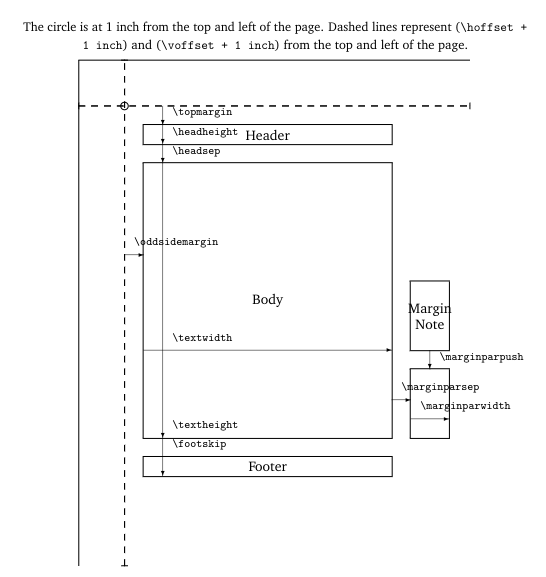
\includegraphics[width=\textwidth]{my-munics-tfm/images/layout.png}
    \caption{Dimensións das marxes utilizadas neste documento}
    \label{fig:layout}
\end{figure}

\paragraph{Tamaño do papel e marxes:} Utilizaráse un tamaño de papel A4, cos valores recomendadas para as marxes mostrados a continuación (véxase a figura \ref{fig:layout}).

\begin{center}
\begin{tabular}{ l l }
\textbackslash paperheight= 845.04694pt & \textbackslash paperwidth= 597.50793pt \\ 
\textbackslash hoffset= 0.0pt & \textbackslash voffset= 0.0pt \\
\textbackslash evensidemargin= 15.45935pt & \textbackslash oddsidemargin= 42.72656pt \\
\textbackslash topmargin= -39.24942pt & \textbackslash headheight= 17.0pt \\
\textbackslash headsep= 20.40001pt & \textbackslash textheight= 636.60028pt \\
\textbackslash textwidth= 394.78204pt & \textbackslash footskip= 185.0pt \\
\textbackslash marginparsep= 12.8401pt & \textbackslash marginparpush= 6.11995pt \\
\textbackslash columnsep= 10.0pt & \textbackslash columnseprule= 0.0pt \\
1em = 10.95pt  & 1ex = 5.2779pt \\
\end{tabular}
\end{center}
%\printinunitsof{cm}{\pagevalues}


\paragraph{Numeración das páxinas:} Tódalas páxinas deben estar numeradas, agás as que non teñan ningún contido ou a páxina de título. As páxinas non numeradas contan ingualmente. Por exemplo, a páxina de título é a  páxina (i).

As páxinas iniciais (o resumo, as dedicacións, a táboa de contidos, etc.) están numeradas con números romanos.  A partir da primeira páxina do primeiro capítulo reiníciase a numeración con números arábigos e continúa consecutivamente ata o final da tese, incluíndo os apéndices.

\paragraph{Espazo entre liñas:} Úsase interliñado simple.  Os parágrafos sepáranse por unha liña en branco (non se sangra a primeira liña do mesmo). 

\paragraph{Títulos e numeración de figuras e táboas:}  Cada táboa, figura, ilustación etc. debe ter un título indicando o elemento que pretende representar ou ilustrar.  As táboas numéranse consecutivamente ao longo do documento. As figuras, ilustracións, etc. tamén se contan consecutivamente ao longo do documento.

\paragraph{Encabezamentos e subtítulos:}     Os títulos indican a organización do documento.     Os capíutulos, secccións e subseccións débense empregar ao longo do documento, sendo coherentes no estilo e posición de cada elemento.  Cada capítulo debe comezar nunha páxina impar. 

\paragraph{Citas bibliográficas:} Débese utilizar un estilo recoñecido (tal como IEEE, APA, etc.). Recoméndase encarecidamente o uso de unha ferramenta como BibLaTeX. 


\section{Organización en seccións}
\label{sec:organización}

Este documento mostra un exemplo da posible organización dunha memoria do TFM. Descríbense a continuación as distintas seccións. 

Non existe un número de páxinas mínimo ou máximo. Non obstante, a extensión dun TFM está habitualmente entre 40 e 80 páxinas. A lonxitude variará segundo o tema elixido e o método de análise, polo que a extensión final deberá ser decidido polo autor e os seus titores. 

Unha posible organización do TFM é a seguinte (as extensións son meramente orientativas): 

\begin{enumerate}[noitemsep]
    \item Páxina de Título (obrigatorio -- 1 páxina).
    \item Resumo en inglés (\textit{abstract} -- obrigatorio -- 1 páxina).
    \item Resumo en galego ou castelán (obrigatorio -- 1 páxina).
    \item Agradecementos (opcional).
    \item Táboa de contidos (obrigatorio).
    \item Introdución (3-10 páxinas).
    \begin{enumerate}[noitemsep]
        \item Motivación.
        \item Obxectivos e presentación do problema que se vai resolver.
        \item Estrutura do documento.
    \end{enumerate}
    \item Situación actual (arpoximadamente 10-20 páxinas). Repaso do traballo relacionado, das tecnoloxías básicas, do punto de partida, etc. 
    \begin{enumerate}[noitemsep]
        \item Traballo relacionado.
        \item Tecnoloxías base.
        \item Marco de traballo (marco teórico, tecnolóxico, etc.).
    \end{enumerate}
    \item Descrición do traballo realizado (aproximadamente 10-20 páxinas). 
    \begin{enumerate}[noitemsep]
        \item Datos analizados.
        \item Análise teórica.
        \item Deseño (arquitectura, ataque, etc.).
        \item Descrición dos métodos. 
        \item Desenvolvementos realizados.
        \item Mecanismos para garantir a calidade do traballo.
    \end{enumerate}
    \item Resultados (aproximadamente 5-20 páxinas)
    \begin{enumerate}[noitemsep]
        \item Descrición dos resultados.
        \item Análise e discusión dos resultados / Validación.
    \end{enumerate}
    \item Conclusións (aproximadamente 5-10 páxinas).
    \begin{enumerate}[noitemsep]
        \item Resumo do traballo.
        \item Implicacións dos resultados / Impacto ecnonómico-social..
        \item Limitacións do traballo.
        \item Traballo futuro.
    \end{enumerate}
    \item Bibliografía (obrigatorio).
    \item Apéndices (opcional).
    \begin{enumerate}[noitemsep]
        \item Descrición de ferramentas.
        \item Descrición de configuración.
        \item Código. 
        \item Detalle adicional para algunha sección. 
        \item Etc. 
    \end{enumerate}
\end{enumerate}



\section{Obxectivos e presentación do problema}
\label{sec:intro:motivación}
{
\color{gray}
\Blindtext[3][1]

\cite{Jurgens:2000,Jurgens:1995,Miede:2011,Kohm:2011,Apple:keynote:2010,Apple:numbers:2010,Apple:pages:2010}

\cite{WEB:GNU:GPL:2010,WEB:Miede:2011}
}

\subsection{Metodoloxía}
\label{sec:intro:results:refs:method}
{
\color{gray}
\Blindtext[1][2]
}

\paragraph{Estratexia 1}
{
\color{gray}
\Blindtext[1][1]
}

\begin{lstlisting}[language=Python, caption={This simple helloworld.py file prints Hello World.}\label{lst:pyhelloworld}]
#!/usr/bin/env python
print "Hello World"
\end{lstlisting}

\paragraph{Estratexia 2}
{
\color{gray}
\Blindtext[1][1]
}

\begin{lstlisting}[language=Python, caption={This is a bubble sort function.}\label{lst:pybubblesort}]
#!/usr/bin/env python
def bubble_sort(list):
    for num in range(len(list)-1,0,-1):
        for i in range(num):
            if list[i]>list[i+1]:
                tmp = list[i]
                list[i] = list[i+1]
                list[i+1] = tmp

alist = [34,67,2,4,65,16,17,95,20,31]
bubble_sort(list)
print(list)
\end{lstlisting}

\section{Organización da memoria}
\label{sec:intro:organización}

\textbf{Capítulo \ref{sec:related}} \\[0.2em]
{
\color{gray}
\blindtext
}

\textbf{Capítulo \ref{sec:system}} \\[0.2em]
{
\color{gray}
\blindtext
}


\textbf{Capítulo \ref{sec:results}} \\[0.2em]
{
\color{gray}
\blindtext
}

\textbf{Capítulo \ref{sec:results}} \\[0.2em]
{
\color{gray}
\blindtext
}

\textbf{Capítulo \ref{sec:conclusion}} \\[0.2em]
{
\color{gray}
\blindtext
}   % INCLUDE: introduction

\chapter{Situación actual} % Estado da arte
\label{sec:related}

\cleanchapterquote{A picture is worth a thousand words. An interface is worth a thousand pictures.}{Ben Shneiderman}{(Professor for Computer Science)}

{
\color{gray}
\Blindtext[2][1]
}

\begin{lstlisting}[language=Java, caption={A simple Hellow World example in Java.}\label{lst:javahelloworld}]
public class HelloWorld {
	public static void main ( String[] args ) {
		// Output Hello World!
		System.out.println( "Hello World!" );
	}
}
\end{lstlisting}

{
\color{gray}
\Blindtext[1][1]
}

\section{Traballo relacionado 1}
\label{sec:related:sec1}

{
\color{gray}
\Blindtext[2][2]
}

\section{Traballo relacionado 2}
\label{sec:related:sec2}
{
\color{gray}
\Blindtext[3][2]
}

\section{Tecnoloxías base}
\label{sec:related:sec3}
{
\color{gray}
\Blindtext[4][2]
}

\section{Marco teórico}
\label{sec:related:conclusion}
{
\color{gray}
\Blindtext[2][1]
}   % INCLUDE: related work

%\part{Exemplo doutra parte}
% !TEX root = ../my-thesis.tex
%
\chapter{Traballo realizado}
\label{sec:system}

\cleanchapterquote{Innovation distinguishes between a leader and a follower.}{Steve Jobs}{(CEO Apple Inc.)}


{
\color{gray}
\Blindtext[2][1]
}

\section{Arquitectura dos desenvolvementos}
\label{sec:system:sec1}
{
\color{gray}
\Blindtext[1][2]
}

\begin{figure}[htb]
	
\includegraphics[width=\textwidth]{images/Clean-Thesis-Figure}
	\caption{Figure example: \textit{(a)} example part one, \textit{(c)} example part two; \textit{(c)} example part three}
	\label{fig:system:example1}
\end{figure}

{
\color{gray}
\Blindtext[1][2]
}

\section{Datos}
\label{sec:system:sec2}

{
\color{gray}
\Blindtext[1][2]
}

\begin{figure}[htb]
	
\includegraphics[width=\textwidth]{images/Clean-Thesis-Figure}
	\caption{Another Figure example: \textit{(a)} example part one, \textit{(c)} example part two; \textit{(c)} example part three}
	\label{fig:system:example2}
\end{figure}

{
\color{gray}
\Blindtext[2][2]
}

\section{Análise teórica}
\label{sec:system:sec3}
{
\color{gray}
\Blindtext[4][2]
}

\section{Deseño}
\label{sec:system:design}
{
\color{gray}
\Blindtext[2][1]
}         % INCLUDE: system

\chapter{Resultados}
\label{sec:results}

\cleanchapterquote{Users do not care about what is inside the box, as long as the box does what they need done.}{Jef Raskin}{about Human Computer Interfaces}


{
\color{gray}
\Blindtext[2][1]
}

\section{Todo é marabilloso}
\label{sec:concepts:sec1}
{
\color{gray}
\Blindtext[2][2]
}

\section{Por que todo é marabilloso?}
\label{sec:concepts:sec2}
{
\color{gray}
\Blindtext[3][2]
}

       % INCLUDE: concepts

\chapter{Conclusións}
\label{sec:conclusion}

{
\color{gray}
\Blindtext[2][1]
}
\section{Resumo}
\label{sec:conclusion:sec1}
{
\color{gray}
\Blindtext[2][2]
}

\section{Implicacións}
\label{sec:conclusion:sec2}
{
\color{gray}
\Blindtext[3][2]
}

\section{Limitacións e traballo futuro}
\label{sec:conclusion:future}
{
\color{gray}
\Blindtext[2][2]
}     % INCLUDE: conclusion

% --------------------------
% Back matter
% --------------------------
%
{%
\setstretch{1.1}
\renewcommand{\bibfont}{\normalfont\small}
\setlength{\biblabelsep}{0pt}
\setlength{\bibitemsep}{0.5\baselineskip plus 0.5\baselineskip}
\printbibliography[]
%\printbibliography[nottype=online]
%\newrefcontext[labelprefix={@}]
%\printbibliography[heading=subbibliography,title={Webpages},type=online]

}
%\cleardoublepage

%\listoffigures
%\cleardoublepage

%\listoftables
%\cleardoublepage

%\lstlistoflistings
%\cleardoublepage

\appendix\cleardoublepage

\chapter{Apéndice}
\label{sec:appendix}

{
\color{gray}
\Blindtext[1][1]
}

\section{Sección 1}
\label{sec:appendix:sec1}

{
\color{gray}
\Blindtext[1][1]

\begin{table}[h]
	\begin{tabularx}{\textwidth}{X | X | X}
		%\hline
		Alpha		& Beta			& Gamma			\\ \hline
		0			& 1				& 2				\\ \hline
		3			& 4				& 5				\\ %\hline
	\end{tabularx}
	\label{tab:table1}
	\caption{This is a caption text.}
\end{table}
}

\section{Sección 2}
\label{sec:appendix:sec2}


{
\color{gray}
\Blindtext[1][1]

\begin{table}[h]
	\begin{tabularx}{\textwidth}{X | X | X}
		%\hline
		Alpha		& Beta			& Gamma			\\ \hline
		0			& 1				& 2				\\ \hline
		3			& 4				& 5				\\ %\hline
	\end{tabularx}
	\label{tab:table2}
	\caption{This is a caption text.}
\end{table}


\Blindtext[1][2]
}       % INCLUDE: appendix


\newpage
\mbox{}

% **************************************************
% End of Document CONTENT
% **************************************************
\end{document}
